\scanpage{587}
\mspage{597}
\[
(51)\qquad
\left\{\begin{aligned}
a&=\varepsilon_3(\tau')\alpha^{-1}u
&\text{i.e.}\quad \alpha&=ua^{-1}\varepsilon_3(\tau')\\
b&=\beta^{-1}u
&\text{i.e.}\quad \beta&=ub^{-1}
\end{aligned}\right.\ ,
\]
je me demande si cette section ensembliste de
$S_0\Gamma_{\rho,\sigma}^{!}$ au dessus de
$Z_{\rho,\sigma}^{!}=M^{!}[0]$ est multiplicative,
\unsure{ou}, ce qui revient au $\overline{\mathrm m}$,
si $a$ et $b$ définis par (51) dépendent multiplicativement de
\deleted{\unsure{ces}} $u$.

\uline{Proposition}. Soit $(u,a,b)\in S_0\Gamma_{\rho,\sigma}^{!}$
(cf (50)). Pour qu'on ait $i=0$, $\unsure{j=0}$, i.e. pour qu'on
ait (51) --- i.e pour que $(u,a,b)$ \deleted{\unsure{soit}}
appartienne à la section ensembliste précédente --- il f. et s.
qu'on ait les relations
\[
(52)\qquad u\equiv b\equiv\varepsilon_3(\sigma)a\,
\deleted{\unsure{(\widehat\Pi_0)}}\quad\bmod\widehat\Pi_0.
\]
\margin{\figure{\begin{tikzpicture}
\draw (0,0)--(0,-2.6);
\end{tikzpicture}}}
\margin{\unsure{où on a posé}
$\displaystyle\varepsilon_3(\sigma)=
\left\{\begin{array}{ll}1&\text{si }\varepsilon_3=+1\\
\sigma&\text{si }\varepsilon_3=-1.\end{array}\right.$}

\margin{\uline{NB}\quad $\tau'\tau=\sigma^{-1}$\quad
$\tau'\sigma^{-1}=\tau$.}

\uline{Démonstration}. Comme
$\beta\deleted{\unsure{\in}}\inserted{=ub^{-1}}$ et
\deleted{$\unsure{\alpha\varepsilon_3(\tau')=ua^{-1}}$}
\inserted{$\deleted{\unsure{\alpha}}\alpha\varepsilon_3(\tau)
=\deleted{\unsure{ua}}ua^{-1}\varepsilon_3(\tau'\tau)
=ua^{-1}\varepsilon_3(\sigma^{-1})$}
sont tous deux dans $\unsure{\widehat\Pi_0}$, la condition est
nécessaire. Pour la suffisance, on note que (52) s'écrit, avec les
notations de (50),
\inserted{\unsure{où} $f=ub^{-1}$, $f'=ua^{-1}$ i.e.
$f'\varepsilon_3(\sigma^{-1})=ua^{-1}\varepsilon_3(\sigma^{-1})$
\deleted{\unsure{soit} $f'\varepsilon_3(\unsure{\sigma})$}}
\deleted{$f,\unsure{f'}\in\Pi_0$},
\inserted{\[
\deleted{\unsure{f\in\Pi_0}}\qquad
(53)\quad f,f'\varepsilon_3(\sigma^{-1})\in\Pi_0
\]
\deleted{\unsure{1}}}
et réduisant mod $\Pi_0$ dans $\unsure{\widehat G}/\Pi_0$
cela s'écrit $\unsure{\dot\beta}\dot\sigma^{i}=1$ et
\deleted{$\unsure{\dot\alpha\dot\rho^{j}\varepsilon_3(\dot\tau)=1}$ i.e.},
\inserted{$\dot\alpha\dot\rho^{j}\varepsilon_3(\tau'\sigma^{-1})^{\cdot}=1$,
cette dernière relation s'écrit aussi
$\dot\alpha\dot\rho^{j}\varepsilon_3(\tau)^{\cdot}=1$ i.e.}
\deleted{cette dernière relation s'écrit aussi}
$\unsure{\varepsilon_3(\dot\tau)\dot\alpha\dot\rho^{j}=1}$,
\deleted{donc la relation devient}
$\varepsilon_3(\dot\tau)\dot\alpha\dot\rho^{j}=1$
or $\varepsilon_3(\dot\tau)\dot\alpha\unsure{=}1$,
la condition est
\deleted{$\varepsilon_3(\dot\tau)\dot\alpha=1$ donc la relation}
\[
\deleted{\unsure{(53)}}\qquad
\dot\sigma^{i}=\dot\rho^{j}=1\qquad\text{i.e.}\quad i=0,\ j=0
\]
\unsure{cqfd}.

\deleted{\uline{Corollaire}\quad La section envisagée est multiplicative.}
\mspage{586}

\scanpage{588}
\deleted{En même temps, ceci nous suggère une modification des constructions
des sections précédentes, en remplaçant les produits fibrés sur
$\unsure{\gamma_{\rho,\sigma}}=
\deleted{\unsure{\Gamma_{\rho,\sigma}\rtimes}}
G_{\rho,\sigma}/\unsure{G}_{\rho,\sigma}^{+}$
par des produits fibrés sur \deleted{$\unsure{\Gamma_{\rho}}$}
le groupe plus fin $G_{\rho,\sigma}/\Pi_0$, qui
\deleted{\unsure{est un}}\inserted{\unsure{dont}} le
\unsure{rev.|gr.} universel est un rev. de degré 12 de celui-ci.}

\unsure{Soient|Soit} maintenant $u$, correspondant à $a,b,\varepsilon_3$
et $u'$, correspondant à $a',b',\varepsilon_3'$, soit
$u''=u'u$, correspondant à $a''$, $b''=b'b$ et
$\varepsilon_3''=\varepsilon_3'\varepsilon_3$, de sorte qu'on aura
\[
\begin{array}{rcll}
u&\equiv&\varepsilon_3(\sigma)a&(\widehat\Pi_0)\\
u'&\equiv&\varepsilon_3'(\sigma)a'&(\unsure{\widehat\Pi_0})\\
u''&\equiv&\underbrace{\varepsilon_3''(\sigma)}a''&(\widehat\Pi_0)\\
\Vert&&&\\[-1ex]
u'u&\equiv&\deleted{\unsure{\varepsilon_3''(\sigma)}}
\varepsilon.\varepsilon_3'(\sigma)\varepsilon_3(\sigma).a''&
\begin{gathered}\text{où }\varepsilon\in\{\pm1\},\ \varepsilon=-1\text{ sss}\\
\varepsilon_3=-1\quad\text{\uuline{et}}\quad\varepsilon_3'=-1
\end{gathered}\\
\vert\!\vert\!\vert&&&\\[-1ex]
(\varepsilon_3'(\sigma)a')(\varepsilon_3(\sigma)a)&&&
\end{array}
\]
\margin{$\unsure{=}$}
\margin{\unsure{!}}

ce qui donne
\[
a'\varepsilon_3(\sigma)a\equiv\varepsilon\varepsilon_3(\sigma)a''
\quad(\widehat\Pi_0)\qquad\text{i.e.}
\]
\[
(53)\qquad a''\equiv\varepsilon\varepsilon_3(\unsure{\sigma})(a').a
\]
\margin{NB $\varepsilon_3(\sigma)$ et $\varepsilon_3(\sigma^{-1})$
opèrent de la $\overline{\mathrm m}$ façon.}

Donc la relation escomptée
\[
a''=a'a\qquad\text{équivalente à}\quad a''\equiv a'a\quad(\widehat\Pi_0)
\]
est vraie si et \uline{seulement si}
\inserted{\deleted{$\unsure{a''=\varepsilon}$}
où $\varepsilon\in\{\pm1\}$ et $\varepsilon=-1$ sss
$\varepsilon_3=\varepsilon_3'=-1$}
\[
(54)\qquad\varepsilon_3(\sigma)(a')\equiv\varepsilon a'
\quad(\widehat\Pi_0)
\deleted{\unsure{(\widehat\Pi_0\tau)}}
\deleted{\unsure{\varepsilon_3(a')=\varepsilon a'}}.
\]
\deleted{ce qui \unsure{pour} $\varepsilon_3$}
\deleted{\unsure{condition qui}}
\deleted{Cette condition se décompose suivant \unsure{les|ces} cas :
$\unsure{\tau'},a'$ sont les images de $\unsure{\tau'},a'$ dans
$\unsure{M}/\widehat\Pi_0$.}
\deleted{\inserted{Cette condition est automatiquement vérifiée}}

\margin{\diagram{\begin{tikzcd}[ampersand replacement=\&,row sep=small,column sep=large]
\deleted{\boxed{54\text{bis}}} \& \\
\deleted{1)\ \varepsilon_3=\varepsilon_3'=1:\ \text{tjrs OK}} \& \\
\deleted{2)\ \varepsilon_3=1,\ \varepsilon_3'=-1:\ \text{tjrs OK}} \& \\
\deleted{3)\ \varepsilon_3=-1,\ \varepsilon_3'=1:\
\boxed{\sigma(a')\equiv a'\ (\widehat\Pi_0)}}
\arrow[r,"\deleted{\text{i.e.}}"] \&
\deleted{\boxed{\sigma(u')\equiv u'\ (\widehat\Pi_0)}}\\
\deleted{4)\ \varepsilon_3=-1,\ \varepsilon_3'=-1:\
\boxed{\sigma(a')\equiv-a'\ (\widehat\Pi_0)}}
\arrow[r,"\deleted{\text{i.e.}}"] \&
\deleted{\boxed{\sigma(u')\equiv-u'\ (\widehat\Pi_0)}}
\end{tikzcd}}}
\mspage{587}

\scanpage{589}
\mspage{598}
\[
(54)\qquad\varepsilon_3(\sigma)(a')\equiv\varepsilon a'
\quad(\unsure{\Pi_0|\widehat\Pi_0}),\quad
\text{où }\left\{\begin{array}{l}
\varepsilon\in\{\pm1\},\quad
\varepsilon\overset{\unsure{\mathrm{dfn}}}{=}-1
\text{ sss }\varepsilon_3=\varepsilon_3'=-1\\
\varepsilon_3(\sigma)\overset{\unsure{\mathrm{dfn}}}{=}
\left\{\begin{array}{ll}1&\text{si }\varepsilon_3=+1\\
\sigma&\text{si }\varepsilon_3=-1\end{array}\right.
\end{array}\right.
\]
Cette condition (54) s'explicite suivant les cas :
\[
(55)\quad\left\{\begin{array}{ll}
a)&\text{si }\varepsilon_3=1,\ \text{alors }\varepsilon=1
\text{ et (54) tjrs vérifiée}\\
b)&\text{si }\varepsilon_3=-1,\ \text{alors (54) s'écrit}\quad
\deleted{\unsure{\varepsilon_3}}\ \sigma(a')\equiv\varepsilon_3'.a'
\quad(\widehat\Pi_0)\quad\text{i.e.}\\
&[\dot\sigma,\dot a']=\dot\varepsilon_3'
\end{array}\right.
\]
\margin{où les $\cdot$ désignent les classes dans $M/\widehat\Pi_0$}

Comme on a
\[
a'\equiv\varepsilon_3'(\sigma)^{-1}u'
=\left\{\begin{array}{ll}
u'&\text{si }\varepsilon_3'=1\\
\sigma^{-1}u'&\text{si }\varepsilon_3'=-1
\end{array}\right.\ ,
\]
on trouve que la condition (55, b) équivaut aussi à :
\[
(56)\quad\deleted{\unsure{[\dot\sigma,\dot u']=\varepsilon_3'}}
\left\{\begin{aligned}
\dot\sigma(\dot u')&=\unsure{\dot\varepsilon_3'|\varepsilon_3'}\dot u'
\quad\text{dans }M/\widehat\Pi_0,\quad\text{i.e.}\\
[\dot\sigma,\dot u']&=\unsure{\dot\varepsilon_3'|\varepsilon_3'}
\end{aligned}\right.
\]
(\inserted{\uline{équivalence}} valable aussi bien pour
$\varepsilon_3'=1$ que $\varepsilon_3'=-1$).

Or on a vu (35) que l'on a dans $\unsure{\widehat G/\widehat\Pi_0}$)
\[
\dot u'(\dot\sigma)=\varepsilon_2(u')\dot\sigma
\]
i.e.
\[
[\dot u',\dot\sigma]=\varepsilon_2(u')\quad\text{ou encore}
\]
\[
(57)\qquad[\dot\sigma,\dot u']=\varepsilon_2(\unsure{\dot u'|\widehat u'})^{\cdot}.
\]
Comparant (56) et (57), on voit que (56) prend la forme équivalente
\[
(58)\qquad\varepsilon_2(u')=\varepsilon_3(u').
\]
On a donc prouvé :

\uline{Proposition}. Soient $u,u'$, et $u''=u'u\in M^{!}[0]=Z_{\rho,\sigma}^{!}$,
correspondants à
$\varepsilon_3\unsure{,|\ne}\varepsilon_3',\
\varepsilon_3''=\varepsilon_3'\varepsilon_3\in\{\pm1\})$, et :
\[
a=\varepsilon_3(\tau')\alpha^{-1}u,\quad
a'=\varepsilon_3'(\tau')\alpha'^{-1}u',\quad
a''=\underbrace{\varepsilon_3''(\tau')}_{\inserted{\varepsilon_3'(\tau')\varepsilon_3(\tau')}}
\alpha''^{-1}\underbrace{u''}_{\inserted{u'u}},
\]
\inserted{avec $a,a',a''\in\unsure{N_\rho'|N_\rho^{*}}$,
$a\equiv\varepsilon_3(\sigma)^{-1}u$, $a'\equiv\ldots$, $a''\equiv\ldots$
$(\Pi_0)$}
\deleted{Pour que} Les conditions suivantes sont équivalentes :

\margin{\uline{NB}\quad
$\displaystyle\left\{\begin{aligned}
\varepsilon_3&=\varepsilon_3(u)=\varepsilon_3(a)\\
\varepsilon_3'&=\varepsilon_3(u')=\varepsilon_3(a')\\
\varepsilon_3''&=\varepsilon_3(u'')=\varepsilon_3(\unsure{a''|a'})
\end{aligned}\right.$}
\mspage{588}

\scanpage{590}
\[
\begin{array}{ll}
a)\ \text{On a}&a''=a'a\\[1ex]
\unsure{a')}\ \text{On a}&a''\equiv a'a\quad(\widehat\Pi_0)\\[1ex]
\unsure{b)}\ \text{On a}&
\varepsilon_3\deleted{\unsure{a}}=1\,
\inserted{\text{i.e. }a(\rho)=\rho}\quad\text{\uline{ou}}\quad
\sigma(a')\equiv\varepsilon_3'a'\quad(\widehat\Pi_0)\\[1ex]
b')\ \text{On a}&
\varepsilon_3=1\,
\inserted{\text{i.e. }a(\rho)=\rho}\quad\text{\uline{ou}}\quad
\unsure{\dot a'|a'}(\sigma)\equiv\varepsilon_3'\sigma
\quad(\unsure{\widehat\Pi_0|\overline\Pi_0})\\[1ex]
c)\ \text{On a}&
\varepsilon_3=1\,
\inserted{\text{i.e. }a(\rho)=\rho}\quad\text{\uline{ou}}\quad
\deleted{\unsure{\varepsilon_3=1}}\ \sigma(\unsure{u'})\equiv
\varepsilon_3'u'\quad(\widehat\Pi_0)\\[1ex]
c')\ \text{On a}&
\varepsilon_3=1\ \inserted{\text{i.e. }a(\rho)=\rho},
\quad\text{\uline{ou}}\quad
\unsure{u'|\dot u'}(\sigma)\equiv\varepsilon_3'\sigma
\quad(\widehat\Pi_0)\\[1ex]
d)\ \text{On a}&
\boxed{\begin{array}{l|l}
\varepsilon_3=1\quad\text{ou}\quad\varepsilon_2'=\varepsilon_3'\quad\text{i.e.}
&\varepsilon_2'\varepsilon_3'=1
\end{array}}
\end{array}
\]

\uline{Corollaire}\quad Au dessus des deux sous-groupes
\[
(59)\quad\left\{\begin{aligned}
\unsure{Z_{\rho,\sigma}^{!'}}&=\unsure{M^{!'}}[0]
\overset{\unsure{\mathrm{dfn}}}{=}
\{u\in Z_{\rho,\sigma}^{!}\mid\varepsilon_3(u)=1\}\\
Z_{\rho,\sigma}^{!'''}&=M^{!'''}[0]
\overset{\unsure{\mathrm{dfn}}}{=}
\{u\in Z_{\rho,\sigma}^{!}\mid\varepsilon_2(u)=\varepsilon_3(u)\}
\end{aligned}\right.
\]
l'application section ensembliste

$(60)\quad A:$
\diagram{\begin{tikzcd}[ampersand replacement=\&,row sep=small,column sep=large]
Z_{\rho,\sigma}^{!}\arrow[r]\arrow[d,equal]
\& S_0\Gamma_{\rho,\sigma}^{!}\\
M^{!}[0]\&\unsure{\ni}\\
\unsure{\cdot}u\arrow[r,mapsto]
\& (u,\ a=\varepsilon_3(\tau')\alpha^{-1}u,\ b=\beta^{-1}u)
\end{tikzcd}}
\margin{cf prop. p. 597}

est une section multiplicative. Mais elle n'est pas multiplicative au
dessus de $\unsure{M^{!}}[0]$ tout entier.
\mspage{589}

\scanpage{591}
\mspage{599}
\uline{Rmque}\quad Les éléments de l'\unsure{image|im.} inverse
$S_0\Gamma_{\rho,\sigma}^{\unsure{!'|'!}}$ de $Z_{\rho,\sigma}^{!'}$
dans $S_0\Gamma_{\rho,\sigma}^{!}$ qui appartiennent à la section envisagée
sont caractérisés (par vertu de la prop. p. 598) par la relation
\[
(61)\qquad u\equiv b\equiv a\quad\bmod\widehat\Pi_0
\]
\margin{(en plus de $\varepsilon_3(u)=1$ qui caractérise les éléments de
$\unsure{S_0\Gamma'_{\rho,\sigma}}$)}
qui rend évident que c'est un ss-groupe.
Je n'ai pas trouvé de jolie expression analogue pour l'appartenance d'un
élément de $S_0\Gamma_{\rho,\sigma}^{\unsure{!'''|!''}}$
(caractérisé par la relation $\varepsilon_2(u)\varepsilon_3(u)=1$)
à la section correspondante.

\uline{Proposition}\quad Soit
$S_0^\Pi\Gamma_{\rho,\sigma}^{!}\subset S_0\Gamma_{\rho,\sigma}^{!}$
le sous-ensemble de $S_0\Gamma_{\rho,\sigma}^{!}$
\deleted{\unsure{de}}
\[
(62)\quad
\begin{gathered}
S_0^\Pi\Gamma_{\rho,\sigma}^{!}\subset S_0\Gamma_{\rho,\sigma}^{!}\\
\unsure{''}\\[-1ex]
\left\{(u,a,b)\in
\begin{array}{c}
\inserted{Z_{\rho,\sigma}\times N_\rho^*\times N_\sigma^*}\\[-.5ex]
\deleted{\unsure{S_0\Gamma_{\rho,\sigma}^{!}}}\\[-.5ex]
\inserted{M[0]}
\end{array}
\ \middle|\ 
\begin{array}{l}
u\equiv b\quad(\widehat\Pi_0)\\
u\equiv\deleted{\unsure{b\equiv}}\varepsilon_3(\sigma)a\quad
\unsure{\bmod}\ \widehat\Pi=\widehat\Pi_0\times\{\pm1\}
\end{array}
\right\}
\end{gathered}
\]
Alors

$a)$ $S_0^\Pi\Gamma_{\rho,\sigma}^{!}$ est un sous-groupe de
$S_0\Gamma_{\rho,\sigma}^{!}$

$b)$ L'\unsure{hom\textsuperscript{om}} \deleted{\unsure{est}}
\diagram{\begin{tikzcd}[ampersand replacement=\&,row sep=small,column sep=large]
S_0^\Pi\Gamma_{\rho,\sigma}^{!}\arrow[r]
\& Z_{\rho,\sigma}^{!}=M^{!}[0],\\
(u,a,b)\arrow[r,mapsto]\&u
\end{tikzcd}}
est surjectif, et son noyau est le sous-groupe, isomorphe à
$\mu=\{\pm1\}$, des éléments $(1,\varepsilon,1)$ avec
$\varepsilon\in\mu=\deleted{\unsure{S_0\Gamma_{\rho}}}
N'_\rho\cap\widehat\Pi=L_\rho\cap\widehat\Pi$
\mspage{590}

\scanpage{592}

\uline{Dém} Le fait qu'on a un sous-groupe résulte du calcul déjà fait p.\ $597',598$, la condition que le produit de deux éléments $(u',a',b')(u,a,b)$ de $S_0^{\Pi}\Gamma_{\rho,\sigma}$ y soit s'exprimant encore par la formule
\[
\tag{56}
[\dot\sigma,\dot u']=\dot\varepsilon'_3
\qquad\text{\uline{dans}}\quad M/\widehat\Pi
\quad(\text{au lieu de }M/\widehat\Pi_0)
\]
\deleted{\unsure{On a}}\inserted{ou} encore
\[
\tag{56 bis}
\begin{gathered}
[\dot u',\dot\sigma]=\dot\varepsilon'_3
\qquad\text{soit}\quad \dot\varepsilon'_3=\dot\varepsilon'_2\\
\unsure{\text{''}}\\
\dot u'(\dot\sigma)\dot\sigma^{-1}=\dot\varepsilon'_2
\end{gathered}
\]
Or dans $\unsure{\widetilde{\mathcal G}|\widetilde{\mathcal C}}/\Pi_0$, \unsure{les} images de $\varepsilon'_2$ et $\varepsilon'_3$ appartiennent toutes deux au sous-groupe central $\Pi/\Pi_0$, donc ils sont triviaux dans $\unsure{\widetilde{\mathcal G}|\widetilde{\mathcal C}}/\Pi$, donc la relation (56 bis) est \unsure{trivialt|trivialement} satisfaite.

La surjectivité de l'application $S_0^\Pi\Gamma^!_{\rho,\sigma}\longrightarrow Z^!_{\rho,\sigma}$ provient du fait que $S_0^\Pi\Gamma^!_{\rho,\sigma}$ contient la section ensembliste $A(Z^!_{\rho,\sigma})$ de la prop. p.\ 597. Le noyau est formé des \deleted{$\unsure{u}$} $(1,a,b)$ avec $a\in N_\rho^*\cap\Pi$, $b\in N_\sigma^*\cap\Pi_0$.

Or $N_\rho^*\cap\unsure{\widetilde{\mathcal G}|\widetilde{\mathcal C}}=\deleted{\unsure{Z_\rho}}L_\rho$, $N_\sigma^*\cap\unsure{\widetilde{\mathcal G}|\widetilde{\mathcal C}}=L_\sigma$, et
\[
\deleted{L_\rho\cap\unsure{\Pi_0|\Pi}=\unsure{\mu}\,L_\sigma\cap\unsure{\Pi}}
\]
\[
\tag{57}
L_\rho\cap\widehat\Pi=L_\sigma\cap\widehat\Pi=\mu,
\qquad L_\rho\cap\widehat\Pi_0=L_\sigma\cap\widehat\Pi_0=\{1\}
\]
\mspage{591}

\scanpage{593}
\mspage{600}

d'où la caractérisation du noyau.

\uline{Corollaire} Considérons \deleted{$\unsure{Z}$} $S_0\Gamma^!_{\rho,\sigma}$ comme une extension de $Z^!_{\rho,\sigma}=M^![0]$ par
\[
\deleted{\unsure{\varepsilon|Z}}\quad
L_\rho\times L_\sigma\simeq\mathbb Z/6\mathbb Z\times\mathbb Z/4\mathbb Z,
\qquad\text{donc}
\]
(en écrivant $L_\rho\simeq\inserted{\mu\times}L_{-\rho}\deleted{\times\unsure{\mu}}\simeq\mathbb Z/3\mathbb Z\times\mathbb Z/2\mathbb Z$)
une extension \unsure{de|des}
\[
\underbrace{\mathbb Z/2\mathbb Z}_{\mu}\times
\underbrace{\mathbb Z/3\mathbb Z}_{L_{-\rho}}\times
\underbrace{\mathbb Z/4\mathbb Z}_{L_\sigma}.
\]

\deleted{L'extension \unsure{co}}

Cette extension \unsure{correspond} donc \unsure{canoniqt|canoniquement} à trois extensions, par $\mu,L_{-\rho},L_\sigma$ respectivement. L\deleted{\unsure{a}}\inserted{'}\deleted{\unsure{section}}\inserted{extension} par $L_{-\rho}\times L_\sigma$ \deleted{\unsure{sont}} \unsure{munie|munies} d'une section canonique.

Il reste une extension (c'est justement $S_0^\Pi\Gamma^!_{\rho,\sigma}$) de $Z^{\unsure{!}}_{\rho,\sigma}$ par $\mu$.

Cette extension correspond \unsure{juste} à l'ambiguïté du signe pour choisir un $\alpha=\widehat\Pi$ au dessus de $\widetilde\alpha\in\widehat\Pi/\pm1$ défini par $u\in Z^!_{\rho,\sigma}=M^![0]$, qui se reflète par l'ambiguïté à choisir le signe pour $a\in\unsure{N'_\rho|N_\rho^*}$, lié à $\alpha$ par (51)
\[
\tag{58}
a=\varepsilon_3(\tau')\alpha^{-1}u,
\qquad \alpha=ua^{-1}\varepsilon_3(\tau'),
\]
Nous avons pu lever cette ambiguïté par l'exigence
$\alpha\in\widehat\Pi_{\unsure{0\tau|0,\tau}}=\deleted{\unsure{\Pi_0}}\{1,\tau\}.\widehat\Pi_0$, et nous

\mspage{592}

\scanpage{594}

venons de constater que ce choix, pour canonique qu'il soit, n'est pas multiplicatif. En $\overline{\mathrm m}$ temps, on trouve l'explicitation complète du $\alpha''$ (\unsure{normalisé} \unsure{canoniqt|canoniquement} par la condition $\alpha''\in\widehat\Pi_{0\tau}$) associé à $u''=u'u$, en termes de $\alpha'$ (associé à $u'$) et $\alpha$ (associé à $u$) également normalisés, \inserted{en termes de $a',a$} En effet, la prop. p.\ 598 nous dit dans quels cas \deleted{\unsure{exacts|exactement}} on a
\[
\tag{59} a''=a'a
\]
savoir sss on a
\[
\tag{59 bis}
\varepsilon_3(u)=1\quad\text{ou}\quad
\varepsilon_{\deleted{\unsure{3|2}}\inserted{2}}(u')\varepsilon_3(u')=1.
\]
Mais on sait maintenant qu'en tous cas on doit avoir
\[
\tag{60}
a''=\varepsilon a'a\qquad \varepsilon\in\{\pm1\}
\]
et on trouve maintenant que $\varepsilon=+1$ sss on est dans le cas (59 bis), $-1$ dans le cas contraire i.e. si $\varepsilon_3(u)=-1$ et $\varepsilon_2(u')\varepsilon_3(u')=+1$. En résumé

\uline{Corollaire} Soient $u,u'\in M^![0]$, d'où $u''=u'u$, soient $\alpha,\alpha',\alpha''\in\widehat\Pi_{0\tau}$ associés (définis par $u(\rho)=\mathrm{int}(\alpha)\rho$ etc) et posons

\mspage{593}

\scanpage{595}
\mspage{601}

\[
\tag{61}
a=\varepsilon_3(\tau')\alpha^{-1}u,\qquad
a'=\varepsilon'_3(\tau')\alpha'^{-1}u',\qquad
a''=\varepsilon''_3(\tau')\alpha''^{-1}u''
\]
où
\[
\varepsilon_3(\tau')=
\begin{cases}
1&\text{si }\varepsilon_3=1\\
\tau'&\text{si }\varepsilon_3=-1
\end{cases}
\qquad
\text{et de }\overline{\mathrm m}\text{ pour }\varepsilon'_3(\tau'),\ \varepsilon''_3(\tau'),
\]
et où $\varepsilon_3=\varepsilon_3(u)=\varepsilon_3(\unsure{\chi|\gamma}(u))$,
et de $\overline{\mathrm m}$ pour $\varepsilon'_3,\varepsilon''_3$
--- donc $\varepsilon''_3=\varepsilon_3\varepsilon'_3$. On a alors
\[
\tag{62}
a''=\varepsilon a'a,\quad\text{avec}\quad\varepsilon\in\{\pm1\}
\]
et
\margin{\deleted{\unsure{et}}\ \unsure{donc}}
\[
\tag{63}
\begin{cases}
\varepsilon=+1&\text{sss}\quad \varepsilon_3=\unsure{1}\ \text{\uline{ou}}\quad
\varepsilon'_2\varepsilon'_3=1\qquad\text{donc}\\
\varepsilon=-1&\text{sss}\quad \varepsilon_3=\unsure{-1}\ \text{et}\quad
\varepsilon'_2\varepsilon'_3=-1.
\end{cases}
\]

On \unsure{aura|a} donc
\deleted{(64)}
\[
\tag{\inserted{*}}
\left\{
\begin{aligned}
\alpha''&=u''a''^{-1}\varepsilon''_3(\tau')\\
&=\varepsilon u'u\,a^{-1}\underbrace{a'^{-1}\varepsilon_3^{\unsure{\deleted{''}|''}}(\tau')}_{\vphantom{A}}\varepsilon'_3(\tau')
\end{aligned}
\right.
\]
et Je \deleted{\unsure{dirais|d'où} $=\varepsilon u'(\alpha)$}
\inserted{\unsure{présume}} qu'on aura
\margin{pas vrai en général}
\[
\tag{64}
\alpha''=\varepsilon u'(\alpha)\alpha'
\qquad\text{où }\varepsilon\text{ donné par (63).}
\]

En effet
\[
\left\{
\begin{aligned}
\alpha&=u\,a^{-1}\varepsilon_3(\tau')\\
\alpha'&=u'\,a'^{-1}\varepsilon'_3(\tau')
\end{aligned}
\right.
\qquad\text{d'où}
\]
\[
\begin{aligned}
u'(\alpha)&=u'u\,a^{-1}\varepsilon_3(\tau')u'^{-1}\\
u'(\alpha)\alpha'&=u'u\,a^{-1}
\underbrace{\varepsilon_3(\tau')\deleted{u'^{-1}}\deleted{u'}a'^{-1}}_{\vphantom{A}}
\varepsilon'_3(\tau')
\end{aligned}
\]
La formule (64), en vertu de (*), prend donc la forme
\[
a'^{-1}\varepsilon_3(\tau')=\varepsilon_3(\tau')a'^{-1}
\]
i.e.
\[
[\varepsilon_3(\tau'),a'^{-1}]=1
\]
elle n'est pas tjrs vérifiée si $\varepsilon_3\deleted{(\unsure{u})}=-1$
i.e.\ $\varepsilon_3(\tau')=\tau'$, où elle représente \inserted{encore} une
restriction draconienne sur $a'$. La formule tjrs correcte est
\deleted{\unsure{(64)|(65)}}
\[
\alpha''=(\varepsilon u'(\alpha)\alpha')\mathbin{.}
\underbrace{\varepsilon'_3(\tau')\bigl([a',\varepsilon_3(\tau')]\bigr)}_{[\varepsilon'_3(\tau')(a'),\,\varepsilon_3(\tau')]}
\]
\mspage{594}

\scanpage{596}

comme $\varepsilon'_3(\tau')a'=\alpha'^{-1}u'$ (61), la formule un \uline{peu alambiquée} :
\margin{Sic ! Voilà le monstre qui m'a fait passer par des sueurs froides
\unsure{pendant} \unsure{une matinée} ou deux !}
\[
\tag{65}
\alpha''=(\varepsilon u'(\alpha)\alpha')\mathbin{.}
\left[
\underbrace{\alpha'^{-1}u'}_{\substack{
\text{''}\\
\varepsilon'_3(\tau')a'\\
\rotatebox[origin=c]{-90}{$\in$}\\
\deleted{\unsure{Z_\rho|N_\rho}}
}},\ \varepsilon_3(\tau')
\right].
\]
(où $\varepsilon\in\{\pm1\}$ \unsure{défini dans|définition} (63))

\unsure{Il|Je} reste à examiner la question si l'extension
\deleted{de} $S_0^{\unsure{\Pi}}\Gamma_{\rho,\sigma}$ de
$Z^!_{\rho,\sigma}\simeq M^![0]$ par $\mu=\{\pm1\}$ est triviale ou non,
tenant compte du fait que ses restrictions à $Z^{!'}_{\rho,\sigma}$ et à
$Z^{!'''}_{\rho,\sigma}$ sont triviales.

Soient $S_0^\Pi\Gamma^{!'}_{\rho,\sigma},\ S_0^\Pi\unsure{\Gamma|W}^{!'''}_{\rho,\sigma}$\unsure{)|]}
les images inv. de $\unsure{Z}^{!'}_{\rho,\sigma},\ Z^{!'''}_{\rho,\sigma}$
dans $S_0^\Pi\Gamma^!_{\rho,\sigma}$, donc
\[
\tag{66}
\left\{
\begin{aligned}
\unsure{S_0^\Pi|\Sigma_{\rho k}^{\Pi}}\Gamma^{!'}_{\rho,\sigma}
&=S_0^\Pi\Gamma^!_{\rho,\sigma}\cap\Gamma^{!'}_{\rho,\sigma}\\
S_0^\Pi\Gamma^{!'''}_{\rho,\sigma}
&=S_0^\Pi\Gamma^!_{\rho,\sigma}\cap\Gamma^{!'''}_{\rho,\sigma}
\end{aligned}
\right.
\]
et on a des suites exactes d'ext. centrales
\diagram{
\[
\tag{67}
\left\{\vcenter{\hbox{%
\begin{tikzcd}[ampersand replacement=\&,column sep=large,row sep=large]
1\arrow[r]\&\mu\arrow[r]\&S_0^\Pi\Gamma^{!'}_{\rho,\sigma}\arrow[r]\&Z^{!'}_{\rho,\sigma}\arrow[r]\&1\\
1\arrow[r]\&\mu\arrow[r]\&S_0^\Pi\Gamma^{!'''}_{\rho,\sigma}\arrow[r]\&Z^{!'''}_{\rho,\sigma}\arrow[r]\&1
\end{tikzcd}%
}}\right.,
\]
}
qui sont scindues par des sous-groupes notés respectivement
$S_0^{\Pi_0}\Gamma^{!'}_{\rho,\sigma},\ S_0^{\Pi_0}\Gamma^{!'''}_{\rho,\sigma}$,
de sorte qu'on a
\[
\tag{68}
\left\{
\begin{aligned}
S_0^\Pi\Gamma^{!'}_{\rho,\sigma}
&\simeq S_0^{\Pi_0}\Gamma^{!'}_{\rho,\sigma}\times\mu\\
S_0^\Pi\Gamma^{!'''}_{\rho,\sigma}
&\simeq S_0^{\Pi_0}\Gamma^{!'''}_{\rho,\sigma}\times\mu.
\end{aligned}
\right.
\]
\mspage{595}

\scanpage{597}
\mspage{602}

Je me pose la question si ces sous-groupes
\[
(69)\qquad
\left\{
\begin{aligned}
S_0^{\Pi_0}\Gamma_{\rho,\sigma}^{!'}&\subset S_0^{\Pi}\Gamma_{\rho,\sigma}^{!'}\subset S_0^{\Pi}\Gamma_{\rho,\sigma}^{!}\\
S_0^{\Pi_0}\Gamma_{\rho,\sigma}^{!'''}&\subset S_0^{\Pi}\Gamma_{\rho,\sigma}^{!'''}\subset S_0^{\Pi}\Gamma_{\rho,\sigma}^{!}
\end{aligned}
\right.
\]
\margin{SS-groupes \unsure{d'indices|d'indice} $4$ dans $S_0^{\Pi}\Gamma_{\rho,\sigma}$}
sont \uline{invariants} dans $S_0^{\Pi}\Gamma_{\rho,\sigma}^{!}$, ce qui
signifierait aussi (\unsure{passant} alors au quotient par ces sous-groupes)
que l'extension $S_0^{\Pi}\Gamma_{\rho,\sigma}^{!}$ de $Z_{\rho,\sigma}^{!}$
par $\mu$, scindée sur $Z_{\rho,\sigma}^{!'}$ et sur $Z_{\rho,\sigma}^{!'''}$,
provient en fait (avec lesdits scindages) d'extensions de
$Z_{\rho,\sigma}^{!}/Z_{\rho,\sigma}^{!'}\ (\simeq\pm1)$ et de
$Z_{\rho,\sigma}^{!}/Z_{\rho,\sigma}^{!'''}\ (\simeq\pm1)$ par $\mu$,
qu'il faudrait ensuite caractériser (comme triviale ou non triviale).

Comme les sous-groupes en question sont distingués dans
$S_0^{\Pi}\Gamma^{!'}$ resp $S_0^{\Pi}\Gamma^{!'''}$, \deleted{et}
si $x$ est un élément de $S_0^{\Pi}\Gamma^{!}$ qui n'est
\uline{pas} dans $S_0^{\Pi}\Gamma^{!'}$ resp $S_0^{\Pi}\Gamma^{!'''}$,
dire que $S_0^{\Pi_0}\Gamma^{!'}$ (resp. $S_0^{\Pi_0}\Gamma^{!'''}$)
est distingué dans $S_0^{\Pi}\Gamma^{!}$ \unsure{tt entier} signifie simplement
qu'il est normalisé par $x$.

$1^\circ)$ Cas de $S_0^{\Pi_0}\Gamma^{!\unsure{'}}\deleted{\unsure{''}}$
dans $S_0^{\Pi}\Gamma^{!}$. On prendra
\inserted{$\underline{x}=(u_0,a_0,b_0)$ avec $u_0=\tau$, d'où
$\varepsilon_3(u_0)=\varepsilon_2(u_0)=\unsure{\chi}(u_0)=-1$,}
\deleted{$x=\tau$, qui n'est pas dans $S_0^{\Pi}\Gamma^{!'}$}
\[
(70)\qquad
\left\{
\begin{gathered}
\alpha_0=\tau,\quad \inserted{\beta_0=1,}\quad
\unsure{a_0}=\unsure{\varepsilon^0_{3,0}}(\tau')\alpha_0^{-1}u_0=\tau',
\quad b_0=\beta_0^{-1}u_0=\tau\big)\\
\text{donc}\qquad
\underline{x}=(\unsure{u_0}=\tau,\ a_0=\tau',\ b_0=\tau)
\end{gathered}
\right.
\]

\mspage{596}

\scanpage{598}

donc on a
\[
x\in S_0^{\Pi_0}\Gamma^{!'''}
\underset{2}{\subset}S_0^{\Pi}\Gamma^{\unsure{!}}
\deleted{\unsure{S_0^{\Pi}\Gamma^{!}}}
\quad\text{et}\quad x\notin S_0^{\Pi}\Gamma^{!'}
\]
et il faut voir si $x$ normalise $S_0^{\Pi_0}\Gamma^{!'}$.

Soit \deleted{$\unsure{u\in}$}
\[
(71)\qquad
\underline{u}\deleted{\unsure{\in Z}}=
\left(
\underset{\inserted{\substack{\rotatebox{90}{$\in$}\\Z}}}{\unsure{u}},
\underset{\inserted{\substack{\rotatebox{90}{$\in$}\\N_\rho'}}}{a},
\underset{\inserted{\substack{\rotatebox{90}{$\in$}\\N_\sigma'}}}{b}
\right)\in S_0^{\Pi_0}\Gamma^{!'}
\quad\text{i.e.}\quad
\left\{\begin{aligned}
u&\equiv a\equiv b\quad(\Pi_0)\\
\varepsilon_3(u)&=1
\end{aligned}\right.
\]
et calculons
\[
\underline{x}\,\underline{u}\,\underline{x}^{-1}
=\underline{x}\,\underline{u}\,x
=(\tau(u),\tau'(a),\tau(b))
\]
est-il dans $S_0^{\Pi_0}\Gamma^{!'}$ (il est dans
$S_0^\Pi\Gamma^{!'}$) i.e. a-t-on
\[
\deleted{\unsure{(70)}}\quad(72)\qquad
\tau(u)\equiv\tau'(\unsure{a})\equiv
\tau^{\deleted{\unsure{'}}}(b)\quad(\Pi_0)\qquad ?
\]
La relation $\tau(u)\equiv\tau(b)\equiv\tau(a)$ est conséquence imm. de
(71), donc (72) équivaut à
\[
\tau'(a)\equiv\tau(a)\quad\inserted{(\Pi_0)}
\qquad(\text{i.e. }\sigma^{-1}(\tau(a))=\tau(a)
\]
i.e.
\[
(73)\qquad\unsure{\text{---}}\qquad
[\dot\sigma,\tau(a)^{\cdot}]=1
\quad\text{dans }\unsure{\widetilde{\mathcal G}^{*}}/\Pi_0
\]
\margin{\uline{NB}}
Ou encore, \deleted{\unsure{évidemment|équivalent}}, en vertu de (35 bis)
\deleted{\[
a=\underbrace{\varepsilon_3(\tau')}_{\substack{\uparrow\\1}}\alpha^{-1}u,
\quad\text{d'où}\quad\tau(a)=\tau(\alpha)^{-1}\tau(u)
\]}
\[
\varepsilon_2(\tau(a))=1\qquad\text{i.e.}\quad\varepsilon_2(a)=1
\]
ou enfin (comme $a\equiv u\ (\Pi_0)$)
\[
(74)\qquad\varepsilon_2(u)=\unsure{1}\,.
\]
Cette condition n'est pas conséquence de la condition $\varepsilon_3(u)=1$,
ce qui montre que $S_0^{\Pi_0}\Gamma^{!'}$ n'est pas invariant dans
$S_0^{\Pi}\Gamma^!$.

$S_0^{\Pi_0}\Gamma^{!'''}$ est-il invariant dans $S_0^{\Pi}\Gamma^!$ ?

Soit \deleted{$x\in S_0$}
\[
(75)\qquad
x=(u_0,\unsure{a_0},b_0)\in S_0^{\Pi_0}\Gamma^{!'}
\mathbin{\setminus}S_0^{\Pi}\Gamma^{!'''}
\quad\text{donc}\quad
\begin{gathered}
\unsure{\text{a)}}\quad
\left\{\begin{aligned}
\varepsilon_3(u_0)&=1\\
\varepsilon_2(u_0)&=-1
\end{aligned}\right.\\
\deleted{\varepsilon_2(u_0)\varepsilon_3(u_0)=\unsure{-1|1}}\\
\text{b)}\quad u_0\equiv b_0\equiv a_0\quad(\Pi_0)
\end{gathered}
\]

\mspage{597}

\scanpage{599}
\mspage{603}

et étudions son action sur
\[
(76)\qquad
\underline{u}=(u,a,b)\in S_0^{\Pi_0}\Gamma^{!'''}
\quad
\left\{\begin{aligned}
\text{a)}\quad
\underbrace{\unsure{\varepsilon_2}(u)}_{\inserted{\varepsilon_2}}
\underbrace{\varepsilon_3(u)}_{\inserted{\varepsilon_3}}&=1\\
\text{b)}\quad u\equiv\unsure{b}&\equiv
\unsure{\varepsilon_3}(\unsure{\sigma})a\quad(\widehat\Pi_0)
\end{aligned}\right.
\]

On a
\[
(77)\qquad
\underline{x}\,\underline{u}\,\underline{x}^{-1}
=(u_0(u),a_0(a),b_0(b))
\]
et la relation $\underline{x}\,\underline{u}\,\underline{x}^{-1}
\in S_0^{\Pi_0}\Gamma^{!'''}$ s'écrit
\[
(78)\qquad
u_0(u)\equiv b_0(b)\equiv\varepsilon_3'(\sigma)\mathbin{.}a_0(a)\,.
\]
\margin{NB $\varepsilon_3(u_0(u))=\varepsilon_3(u)$}
Or les relations (75) b) et 76 b) impliquent aussitôt
\[
u_0(u)\equiv b_0(b)\equiv
\underbrace{a_0(\varepsilon_3(\sigma)\mathbin{.}a)}_{
\varepsilon_3[a_0(\sigma)]\mathbin{.}a_0(a)}
\]
donc la relation (78) équivaut aussi à
\[
(79)\qquad
\varepsilon_3[\sigma]\equiv\varepsilon_3[a_0(\sigma)]
\]
ce qui est automatiquement vérifié si $\varepsilon_3=1$, et pour
$\varepsilon_3=-1$ revient à
\[
(80)\qquad\sigma\equiv a_0(\sigma)\quad\unsure{(\widehat\Pi_0)}
\]
\[
\text{i.e.}\quad\varepsilon_2(a_0)=1\qquad
\text{i.e.}\quad\varepsilon_2(u_0)=1,
\]
relation qui est \uline{fausse} par l'hyp. 75 a).

Donc on trouve encore $S_0^{\Pi_0}\Gamma^{!'''}$ \unsure{non-invariant}
dans $S_0^{\Pi}\Gamma^!$. Par contre,
\deleted{\unsure{désignons|définissons}}\inserted{posons}
\deleted{par $\Gamma^0$ le}
\[
(81)\qquad
\left\{\begin{aligned}
S_0\Gamma^0
&=\operatorname{Ker}\bigl(S_0\Gamma^0
\xrightarrow{(\varepsilon_2,\varepsilon_3)}\mu\times\mu\bigr)
=S_0\Gamma^{!'}\cap S_0\Gamma^{\unsure{!'''}}\\
&\hspace{22em}=S_0\Gamma^{!'}\cap S_0\Gamma^{!''}\\
&\hspace{22em}=S_0\Gamma^{!''}\cap S_0\Gamma^{!'''}\\
S_0^{\Pi}\Gamma^0&=S_0\Gamma^{!0}\cap S_0^{\Pi}\Gamma^!,\\
S_0^{\Pi_0}\Gamma^0&=S_0\Gamma^{!0}\cap S_0^{\Pi_0}\Gamma^!,
\end{aligned}\right.
\]
\margin{\deleted{\unsure{b)}}}
de sorte qu'on a une suite exacte
\[
(82)\qquad
\diagram{\begin{tikzcd}[ampersand replacement=\&,column sep=large]
1\arrow[r,dash]\&\mu\arrow[r,dash]\&
S_0^{\unsure{\Pi|\Pi_0}}\Gamma^{\unsure{!0}}
\arrow[r]\&S_0\Gamma^{!0}\arrow[r]\&1
\end{tikzcd}},
\]

\mspage{598}

\scanpage{600}

canoniquement scindée par $S_0^{\Pi_0}\Gamma_0$ --- on trouve donc
\[
(82)\qquad
S_0^{\Pi}\Gamma^{!0}=S_0^{\Pi_0}\Gamma^{!0}\times\mu\,.
\]

Ceci posé, les calculs précédents montrent que
$S_0^{\Pi_0}\Gamma^{!0}$, qui est d'indice $8$ dans
$S_0^{\Pi}\Gamma^!$, est un sous-groupe invariant. En résumé:

\uline{Proposition} Considérons les sous-groupes
\inserted{(d'indices $4,4,8$)}
\deleted{de}
$S_0^{\Pi_0}\Gamma^{!'},\ S_0^{\Pi_0}\Gamma^{!'''},\
S_0^{\Pi_0}\Gamma^{!0}$ de $S_0^{\Pi}\Gamma^!$ qui sont les images
\unsure{des|de leurs} restrictions \inserted{homomorphiques}
$Z^{!'},Z^{!'''},Z^{!0}$ de la section ensembliste:
$A$ définie par (51) (52) de $S_0^{\Pi}\Gamma^!$ sur
$Z=M[0]$ --- qui est multiplicative sur ces sous-groupes,
et définit donc des scindages des images inverses
$S_0^{\Pi}\Gamma^{\unsure{'|!'}},
S_0^{\Pi}\Gamma^{\unsure{'''|!'''}},
S_0^{\Pi}\Gamma^{\unsure{0|!0}}$
de \deleted{$\unsure{S_0^{\Pi}}$}
$Z^{!'},Z^{!'''},Z^{!0}$ dans $S_0^{\Pi}\Gamma^!$:
\[
(83)\qquad
\begin{gathered}
S_0^{\Pi}\Gamma^{!'}\simeq
\deleted{\unsure{\mu}}S_0^{\Pi_0}\Gamma^{!'}\times\mu,\qquad
S_0^{\Pi}\Gamma^{!'''}=S_0^{\Pi_0}\Gamma^{!'''}\times\mu,\qquad
S_0^{\Pi}\Gamma^{!0}=S_0^{\Pi_0}\Gamma^{!0}\times\mu.
\end{gathered}
\]

\margin{\figure{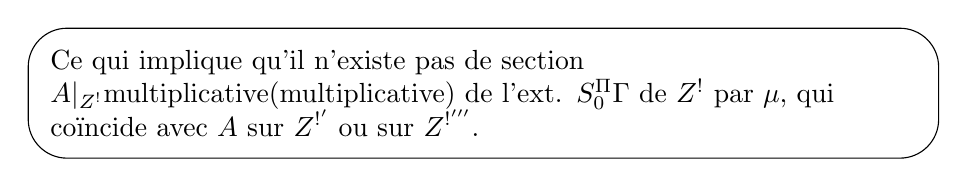
\begin{tikzpicture}
\node[draw,rounded corners=14pt,inner sep=8pt,text width=11cm,align=left]
{Ce qui \unsure{implique} qu'il n'existe pas de section
\deleted{$\unsure{A|_{Z^!}}$\unsure{multiplicative}}\inserted{(multiplicative)}
de l'ext. $S_0^{\Pi}\Gamma$ de $Z^!$ par $\mu$, qui coïncide
avec $A$ sur $Z^{!'}$ ou sur $Z^{!'''}$.};
\end{tikzpicture}}}

On a alors ceci:

a) $S_0^{\Pi_0}\Gamma^{!'},S_0^{\Pi_0}\Gamma^{!'''}$ ne sont
\uline{pas} \uline{distingués} dans $S_0^{\Pi}\Gamma^!$.

b) $S_0^{\Pi_0}\Gamma^{!0}$ est distingué dans
$S_0^{\Pi}\Gamma^!$, de sorte que l'ext.
$S_0^{\Pi}\Gamma^!$ de $Z^!\simeq M^![0]$ par $\mu$
est canoniquement isom. à l'image inverse d'une
\unsure{catégorie|extension} \inserted{centrale} finie
$S_0^{\Pi}\Gamma^!/(S_0^{\Pi_0}\Gamma^{!0})$
de $Z^!/Z^{!0}\simeq\mu\times\mu$ par $\mu$.

\mspage{599}

\scanpage{601}
\mspage{604}

Examinons cette extension centrale
\[
(84)\qquad
\diagram{\begin{tikzcd}[ampersand replacement=\&,column sep=large,row sep=small]
1\arrow[r]\&\mu\arrow[r]\&
\mathcal E\arrow[r,"{(\varepsilon_3,\varepsilon_2)}"]
\arrow[d,phantom,"{\rotatebox{90}{$\simeq$}}" description]\&
\mu\times\mu\arrow[r]\&1\\
\&\&S_0^\Pi\Gamma_{\rho,\sigma}/S_0^{\Pi_0}\Gamma^0_{\rho,\sigma}\&\&
\end{tikzcd}}
\]
s'insérant dans le diagramme d'extensions,
\[
(85)\qquad
\diagram{\begin{tikzcd}[ampersand replacement=\&,column sep=large,row sep=large]
1\arrow[r,dash]\&\mu\arrow[r]\&
\mathcal E\arrow[r,dash]\&\mu\times\mu\arrow[r,dash]\&1\\
1\arrow[r,dash]\&\mu\arrow[r]\arrow[u,"1"']\arrow[d,hook]\&
S_0^\Pi\Gamma^!_{\rho,\sigma}\arrow[r]\arrow[u]\arrow[d,hook]\&
Z^!_{\rho,\sigma}\arrow[u,"{(\varepsilon_3,\varepsilon_2)}"']
\arrow[d,leftrightarrow,"1"]\arrow[r,phantom,"{\simeq M[0]}" description]\&\vphantom{1}\\
1\arrow[r]\&L_\rho\times L_\sigma\arrow[r]\&
S_0\Gamma^!_{\rho,\sigma}\arrow[r,dash]\&Z^!_{\rho,\sigma}\arrow[r]\&1
\end{tikzcd}}
\]

L'intérêt de (84) est qu'elle permet de récupérer l'extension
$S_0\Gamma_{\rho,\sigma}$ de $Z^!_{\rho,\sigma}$ par
$L_\rho\times L_\sigma$, par la \unsure{loi}
\unsure{covariante}-\unsure{contravariante} dans le foncteur
``extensions'', de
\[
(86)\qquad
\diagram{\begin{tikzcd}[ampersand replacement=\&,column sep=large,row sep=small]
Z^!_{\rho,\sigma}\arrow[r,"{(\varepsilon_3,\varepsilon_2)}"]\&
\mu\times\mu
\end{tikzcd}},\qquad
\begin{gathered}
\diagram{\begin{tikzcd}[ampersand replacement=\&,column sep=large,row sep=small]
\mu\arrow[r,hook]\&L_\rho\times L_\sigma\\
-1\arrow[r,mapsto]\&(\rho^3,\sigma^2)
\end{tikzcd}}\\
\text{(``hom. diagonale'')}
\end{gathered},
\]
ainsi que la sous-extension $S_0^\Pi\Gamma^!_{\rho,\sigma}$ de
celle-ci (de $Z^!_{\rho,\sigma}$ par $\mu$).

Étudions d'abord l'ordre des éléments de $\mathcal E$ --- ils sont
évidemment diviseurs de $4$, sont ils tous d'ordre $2$ (ou $1$)? Soit
\[
\underline{\unsure{\bar u|u}}=
\left(
\underset{\inserted{\substack{\rotatebox{90}{$\in$}\\Z}}}{u},
\underset{\inserted{\substack{\rotatebox{90}{$\in$}\\N_\rho^*}}}{a},
\underset{\inserted{\substack{\rotatebox{90}{$\in$}\\N_\sigma^*}}}{b}
\right)\in S_0^\Pi\Gamma^!
\qquad\text{i.e.}\quad
\left\{\begin{aligned}
u&\equiv b\quad(\widehat\Pi_0)\\
u&\equiv\varepsilon_3[\sigma]a\quad(\widehat\Pi)
\end{aligned}\right.
\qquad(87)
\]
\margin{\uline{NB} Pour \unsure{interdire|introduire} des confusions,
\unsure{j'écris} $\varepsilon_3[\sigma],\varepsilon_3[\tau']$
de préférence \unsure{à|de} $\varepsilon_3(\sigma),\varepsilon_3(\tau')$
pour $\sigma^{\unsure{\nu_3}},\tau'^{\unsure{\nu_3}}$.}

Je \deleted{\unsure{veux}} veux examiner si
$\underline{u}^{2}\in S_0^{\Pi_0}\Gamma^{!0}$.
Évidemment
\[
\underline{u}=(u^2,a^2,b^2)\in S_0^\Pi\Gamma^{!0}
\]

\mspage{600}

\scanpage{602}

il reste à voir si $\underline u^{2}\in S_0^{\Pi_0}\Gamma^{!}$, i.e. si on a
\deleted{\unsure{non}} seulement
$\unsure{u^{2}}\equiv b^{2}\ (\Pi_0)$ et
$\deleted{\unsure{a^{2}}}\unsure{u^{2}}\equiv a^{2}\ (\widehat\Pi)$
--- ce qui est clair et exprime simplement
$\underline u^{2}\in S_0^{\Pi}\unsure{\Gamma|\Gamma^{!}}$ --- mais même
\[
\tag{88}
\unsure{u^{2}}\equiv a^{2}\quad\bmod\ \uuline{\widehat\Pi_0}
\qquad (?)
\]

La relation
\[
u\equiv\varepsilon_3[\sigma].a\quad\bmod\Pi
\]
s'écrit aussi
\[
u\equiv\pm\varepsilon_3[\sigma].a\quad\bmod\Pi_0
\]
et implique
\[
u^2\equiv\varepsilon_3[\sigma]a\ \varepsilon_3[\sigma]a
\quad\bmod\Pi_0
\]
ce qu'on peut écrire
\[
\tag{89}
\underset{\bmod\widehat\Pi_0}{u^2\equiv
\varepsilon_3\,\varepsilon_3[\sigma](a).a}
=\begin{cases}
a^2&\text{si }\varepsilon_3=1.\\
-\sigma(a).a&\text{si }\varepsilon_3=-1
\end{cases}
\]

Donc (88) est vraie si $\varepsilon_3=1$, tandis que
pour $\varepsilon_3=-1$, elle équivaut à
\[
\sigma(a)\equiv-a\qquad(\widehat\Pi_0)
\]
i.e.
\[
[\sigma,a]^{\cdot}=-1\quad\text{dans }\unsure{\widetilde{\mathcal G}|\widetilde{\mathcal C}}/\Pi_0
\]
i.e.
\[
\underbrace{\varepsilon_2(a)}_{\inserted{\begin{gathered}\rotatebox{90}{$=$}\\\varepsilon_2(u)\end{gathered}}}=-1
\qquad\text{i.e. }\varepsilon_2(\unsure{u})\varepsilon_3(\unsure{u})=1.
\]

Donc on trouve :

\uline{Proposition} Soit $x\in\mathcal E$ (cf (84)). Pour que
l'on ait $x^2=1$, il f. et s. qu'on ait
$\varepsilon_3(x)=1$ \uline{ou} $\varepsilon_2(x)\varepsilon_3(x)=1$,
i.e. que
\deleted{$x$ \unsure{appartienne au sous-groupe} $\mathcal E'$ \unsure{ou}}
\inserted{l'on ait}
\[
\tag{90}
x\in\mathcal E'\cup\mathcal E''',
\]

\mspage{601}

\scanpage{603}
\mspage{605}

où
\[
\tag{91}
\mathcal E'=\{\unsure{x|n}\in\mathcal E\mid\varepsilon_3(x)=1\},\qquad
\mathcal E'''=\{\unsure{x|n}\in\mathcal E\mid\varepsilon_2(x)\varepsilon_3(x)=1\}
\]

\uline{Corollaire 1} $\mathcal E$ a exactement deux éléments
d'ordre $4$, qui sont les deux éléments de $\mathcal E$ au
dessus de l'élément $(-1,1)$ de $\mu\times\mu$.
Ces deux éléments sont inverses l'un de
l'autre, \unsure{ce|et} sont les deux générateurs du
seul sous-groupe cyclique d'ordre $4$ de $\mathcal E$,
qui n'est autre que
\[
\tag{92}
\mathcal E''=\{\unsure{x|n}\in\mathcal E\mid\varepsilon_2(x)=1\}
\]

\uline{Corollaire 2} L'extension $\mathcal E$ n'est pas scindée.

Car étant centrale, elle \deleted{\unsure{se}} serait isomorphe
à $(\mu\times\mu)\times\mu$, donc ses éléments seraient d'ordre
qui divise $2$.

Nous pouvons regarder maintenant
$\mathcal E$ comme extension de $\mathcal E/\mathcal E''\simeq\{\pm1\}=\mu$ par
$\mathcal E''\ (\simeq\mathbb Z/4\mathbb Z)$.
\deleted{Mais il} Il faudrait
d'abord expliciter l'opération de $\mathcal E/\mathcal E''=\mu$
sur $\unsure{\mathcal E'|\mathcal E''}$ --- l'élément \inserted{$-1$} d'ordre $2$ de $\mu$
induit un \unsure{autom.} involutif de \deleted{$\unsure{\mathbb Z/4\mathbb Z}$} $\mathcal E''$
\inserted{d'ailleurs dans $\mathrm{Aut}(\unsure{\mathcal E'|\mathcal E''})\simeq
(\mathbb Z/4\mathbb Z)^*\simeq\{\pm1\}$, donc
l'autom. en question}
\deleted{que \unsure{son}} est la multiplication par un
signe $\varepsilon\ \pm1$, qu'il faut déterminer. On va
prendre \inserted{comme représentant de $-1\in\mathcal E/\mathcal E''$}
l'élément de $\mathcal E$ provenant
\deleted{de}\inserted{de}
\[
\tag{92}
\deleted{\unsure{\tau,a',\tau}}\quad
\underline x=(u_0=\tau,\ a_0=\tau',\ b_0=\tau)
\in S_0^{\Pi_0}\Gamma^{!'''}\qquad(\text{cf}(70))
\]
qu'on va faire opérer sur l'image d'un
\[
\tag{93}
\underline u=(u,a,b)\in S_0^{\Pi}\Gamma^{!},\quad
\deleted{\unsure{\text{avec}}}\ \text{où }\varepsilon_3(u)=-1,\ \varepsilon_2(u)=1
\]
\inserted{\[
\left(\begin{array}{ll}
u\equiv b\ \deleted{\unsure{\equiv a}}&\bmod\widehat\Pi_0\\
u\equiv\sigma a&\bmod\widehat\Pi
\end{array}\right)
\]}
(qui est un générateur de $\mathcal E''$).

\mspage{602}

\scanpage{604}

On aura donc
\[
\underline x(\underline u)=(\tau(u),\tau'(a),\tau(b))\equiv
\deleted{\unsure{(u,\varepsilon a,\varepsilon b)|(\varepsilon u,\varepsilon a,\varepsilon b)}}
\underbrace{\inserted{(1,\varepsilon,\varepsilon)(u,a,b)}}_{\inserted{(u,\varepsilon a,\varepsilon b)}}
\]
mod $S_0^{\Pi_0}\Gamma^{\unsure{!0|0}}$, avec un signe
$\varepsilon\in\{\pm1\}$ à déterminer. La condition de congruence s'écrit
\[
(u\tau(u)^{-1},\ \varepsilon a\tau'(a)^{-1},\
\varepsilon b\unsure{\tau'(b)|\tau(b)}^{-1})\in S_0^{\Pi_0}\Gamma^{\unsure{!0|0}}
\]
qu'on soit dans $S_0^\Pi\Gamma^{!0}$ est évident,
\deleted{\unsure{le choix}}
\deleted{\unsure{indifférent|indépendant}}
\inserted{\unsure{valble|valable}}
quel que soit le choix du signe
$\varepsilon$, \deleted{\unsure{c'est}}
\deleted{\unsure{c'est|et}}\inserted{\unsure{c'est}}
\unsure{la|les} \unsure{condition|conditions} de congruence
\deleted{qui} \deleted{\unsure{sont essentielles}}
\inserted{qui \unsure{distingue|distinguent} $S_0^{\Pi_0}\Gamma^{!}$ de
$S_0^\Pi\Gamma^{!}$ qui est}
essentielle, savoir
\[
\tag{94}
u\tau(u)^{-1}\equiv\varepsilon\unsure{a}\tau'(\unsure{a})^{-1}
\qquad(\widehat\Pi_0)\qquad\text{soit}
\]
\deleted{\[
\unsure{u(\tau)\tau^{-1}\equiv\varepsilon a(\tau')\tau'^{-1}}
\]}

La difficulté avec cette approche vient
du fait que les seuls éléments de
$M$ qu'on sache expliciter sont ceux qui
proviennent de $\unsure{\widetilde{\mathcal G}|\widetilde{\mathcal C}}\simeq\mathrm{Gl}(2,\mathbb Z)$
lui-$\overline{\mathrm m}$ ; or
pour ceux-ci on a $\varepsilon_2(u)\varepsilon_3(u)=1$, alors
que le $u$-\inserted{ici} \deleted{\unsure{test}} ci-dessus doit satisfaire
$\varepsilon_2(u)=1$, $\varepsilon_3(u)=-1$ donc
$\varepsilon_2(u)\varepsilon_3(u)=-1$.
On \unsure{peut} d'autre part travailler dans le
\deleted{\unsure{\text{groupe}} $\unsure{\widetilde{\mathcal G}|\widetilde{\mathcal C}}$}
\inserted{quotient} $\mathrm{Gl}(2,\widehat{\mathbb Z})$ de
\deleted{$\unsure{\widetilde{\mathcal G}|\widetilde{\mathcal C}}$} $M$, et
y prendre
\[
\tag{95}
u=\begin{pmatrix}\mu&0\\0&1\end{pmatrix}
\quad\text{avec}\quad
\mu\in\widehat{\mathbb Z}^{*},\quad
\begin{cases}
\mu\equiv-1&(3)\\
\mu\equiv1&(4)
\end{cases}
\]
\inserted{\[\text{i.e.}\quad\mu\equiv5\quad(12)\]}
tandis que $\tau$ correspond à la
matrice
\[
\tau=\begin{pmatrix}-1&0\\0&1\end{pmatrix}
\]

\margin{$\unsure{\wedge}$}
\mspage{603}

\scanpage{605}
\mspage{606}

on aura de toutes façons
\[
u\tau(u)^{-1}=1
\]
soit d'autre part dans $\mathrm{Gl}(2,\widehat{\mathbb Z})$
\[
\tag{96}
\left\{\begin{array}{lll}
a=\tau'a_0&a_0=c\rho+d&c^2+cd+d^2\in\widehat{\mathbb Z}^{*}\\[3pt]
&\tau'=\begin{pmatrix}0&1\\1&0\end{pmatrix},&
\rho=\begin{pmatrix}0&1\\-1&1\end{pmatrix}
\end{array}\right.
\]
\unsure{donc|d'où}
\[
\tag{97}
a=\begin{pmatrix}0&1\\1&0\end{pmatrix}
\begin{pmatrix}d&c\\-c&c+d\end{pmatrix}
=\begin{pmatrix}-c&c+d\\d&c\end{pmatrix}
\]
et
\[
\tag{98}
\mu=-(c^2+cd+d^2)
\]

\margin{\unsure{un peu bref}... cf plus bas...}

On \deleted{\unsure{va}} travailler avec le \inserted{sous-}groupe fermé
$\widehat\Pi_0$ dans $\mathrm{Sl}(2,\widehat{\mathbb Z})$ engendré par
\[
\begin{gathered}
-\ell_0\underset{\unsure{,}}{\unsure{=}}\unsure{-}\begin{pmatrix}
1&-2\\\deleted{\unsure{-2|2}}0&1
\end{pmatrix},\qquad
-\ell_1=-\begin{pmatrix}1&0\\\unsure{2|1}&\unsure{1|0}\end{pmatrix},\qquad
-\ell_\infty=-\begin{pmatrix}3&-2\\2&-1\end{pmatrix}
\end{gathered}
\]
et dans le groupe quotient de
$\mathrm{Gl}(2,\widehat{\mathbb Z})$ par $\widehat\Pi_0$, qui est
\deleted{\unsure{l'}} l'extension de
$\widehat{\mathbb Z}^{*}$ par
\[
\mathrm{Sl}(2,\widehat{\mathbb Z})/\widehat\Pi_0
\simeq\mathrm{Sl}(2,\mathbb Z)/\Pi_0
\simeq\left\{(\rho,\sigma)\ \left|\begin{array}{l}
\rho^6=\sigma^4=1\\
\rho^3=\sigma^2\\
\sigma(\rho)=\rho^{-1}
\end{array}\right.\right\},
\]
\deleted{\unsure{avec}} et \unsure{ce|en} produit $\frac12$ direct grâce à
\[
T_0=\left\{\begin{pmatrix}
\deleted{\unsure{\xi}}\unsure{\zeta|\xi}&0\\0&1
\end{pmatrix}\ \middle|\ \unsure{\zeta|\xi}\in\widehat{\mathbb Z}^{*}\right\}
\overset{\det}{\simeq}\widehat{\mathbb Z}^{*},
\]
opérant par l'intermédiaire de $\varepsilon_2(\unsure{\zeta|\xi})$
--- cf p. $593'$, $594$ --- formules (34)(35)(35 bis) ].
On \inserted{doit} supposer
\[
\tag{99}
\sigma a\equiv u\qquad(\widehat\Pi_{\unsure{0}})
\qquad\text{où }\sigma=\begin{pmatrix}0&-1\\1&0\end{pmatrix}
\]
donc
\[
\tag{100}
\sigma a=\begin{pmatrix}-d&-c\\-c&c\unsure{+}d\end{pmatrix}
\]

\mspage{604}
